\documentclass{projdoc}

\title{Research Document}

\begin{document}
\tablestables
\newpage

% \section{Introduction}

\section{Game engine}

\subsection{Introduction}

To build a game engine, it must first be understood how it operates. The
functionalities it requires and how these functionalities work together must be
determined. In this section, the general functioning of a game engine and the
different parts required are described.

\subsection{Findings}

A game engine is not the game itself but a platform with which games are built. It
should provide the functionalities with which the game is constructed. The purpose of
a game engine is not to create data out of nothing. Instead, data is read, and the
correlating features and effects are generated. However, the engine is also used to
create these files, referred to as ``assets''. The game engine must be able to accept
a certain format of these assets---whether levels, sprites, or textures---and convert
them into usable data.

\subsubsection{Layers}

A game engine is composed of multiple layers, each with its own functions. These
layers are divided into the following categories:\noparbreak
\begin{description}
	\item[Resource manager] Responsible for what happens when the engine is launched,
		including loading data formats.
	\item[Application] Manages the run loop, time, code execution, and events
		(e.g.~input events).
	\item[Window/\glspl{hid}] Handles input and events.
	\item[Renderer] Responsible for drawing the necessary objects on the screen,
		usually once per frame.
	\item[Debugging support] Provides testing for the engine, such as logging or
		performance profiling.
	\item[Scripting layer] Runs scripts, such as Lua or Python.
	\item[Memory systems] Handles and monitors memory usage.
	\item[Physics] Adds specific physics to objects.
	\item[Audio] Processes audio.
	\item[AI] Provides artificial inteligent behavior.
\end{description}

\subsubsection{Structures}

The above mentioned layers should be structured, somehow. One of the requirements is
that the game engine's API uses a so-called gameObject (with one or more
component(s)). The gameObject is described in more detail at
\cref{sec:gameobjects-components}.

There are multiple structures that could be used to structure a game engine. It's of
course possible to use inheritance. A major disadvantages of inheritance is that it's
not flexible. However, the provided class diagram of the game engine's API already
specifies that composition should be used (in stead of inheritance). So, let's take a
look at structures that use composition.

The Decorator design pattern (as shown in \cref{fig:decorator}) could be used to
structure the game engine. A gameObject's propperties/behavior is determined by one
(or more) components. The Decorator design pattern allows to modify an object's
propperties/behavior by adding one (or more) Decorators. The object that is modified,
could be the gameObject and the components could be the Decorators. This is not
exactly the same as the required API, but it's very close. A major disadvantage of
such Decorator design pattern, is that the interface of all components should be the
same (they should share the same methods), because the client (which is the scene in
our case) can only call/reach the components through the interface. This would
require very general methods (at the interface), which might make the programming
harder \autocite{man:DecoratorDesignPattern}.

\begin{figure}
	\centering
	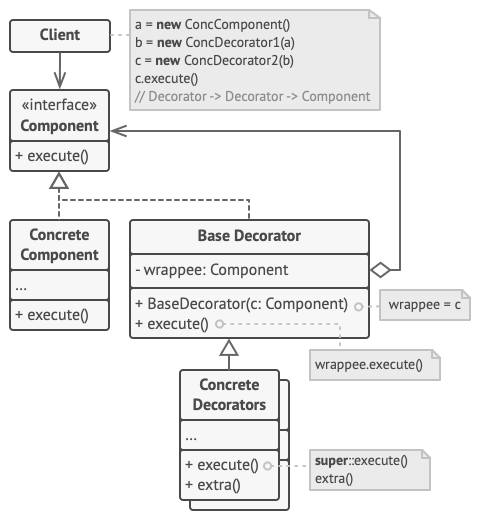
\includegraphics[width=0.5\textwidth]{img/DecoratorDesignPattern.png}
	\caption{Decorator design pattern}
	Source: \autocite{img:Decorator}
	\label{fig:decorator}
\end{figure}

The \emph{extension objects} design pattern (as shown in \cref{fig:dp:ext-objs})
could also be used to structure the game engine. The extension objects design pattern
allows to modify an object's propperties/behavior by adding one (or more) Extensions.
The object that is modified, could be the gameObject and the components could be the
Extensions. This is quite the same as the required API. An advantage is, that the
client (which is the scene in our case) can call all kind of different Extension's
methods (depending on the kind of Externsion, e.g.~the method \codeinline{render()}
for the sprite Extension and the method \codeinline{update()} for the script
Extension). In other words, the interfaces of the different Extensions should not be
the same. This is way more flexible than the Decorator design pattern. A disadvantage
is that the data and functionality are in the same class (namely inside the Extion's
methods), so it's not sepperated. Another disadvantage is that the extension objects
design pattern can be quite slow, because objects are scattered in memory (and it is
very hard to quickly get their memory address)
\autocite{man:ExtensionObjectDesignPattern, man:extionsionObjectsStackOverflow}.

\begin{figure}
	\centering
	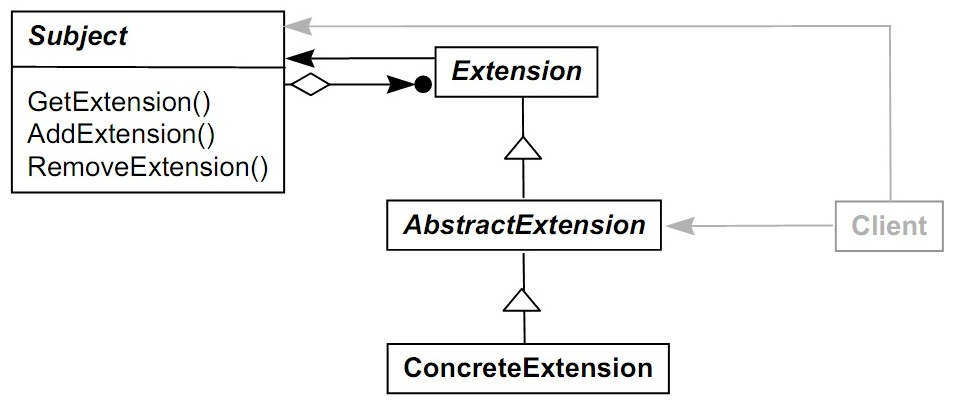
\includegraphics[width=0.5\textwidth]{img/ExtensionObjects.jpg}
	\caption{Extension objects design pattern}
	Source: \autocite{img:extionsionObjects}
	\label{fig:dp:ext-objs}
\end{figure}

Another (very popular) design pattern to structure the game engine, is the Entity
Component System (\gls{ecs}) (as shown in \cref{fig:ECS Block Diagram}). The
\gls{ecs} is made out of three main subsystems, namely entities, components and
systems. Entities are just IDs. An entity is made out of a gameObject and one (or
more) components. Components are the classes that hold the data. The components
determine what kind of entity it is (e.g.~a sprite, audio, and so on). Systems take
care of the behavior of the entities. Systems mainly read and write the enity's
components data. The \gls{ecs} clearly distinguishes the data (components) from the
functionality (systems), which is an advantage.

\begin{figure}
	\centering
	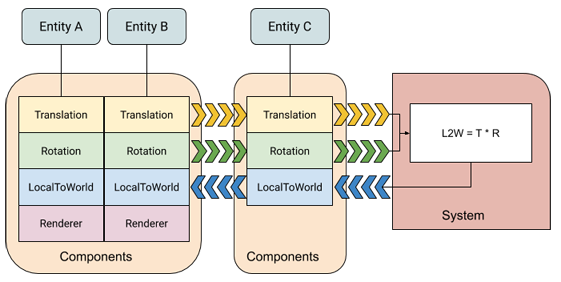
\includegraphics[width=0.5\textwidth]{img/ECSBlockDiagram.png}
	\caption{ECS design pattern}
	Source: \autocite{img:ECSBlockDiagram}
	\label{fig:ECS Block Diagram}
\end{figure}

The \gls{ecs} is normally equipped with a component manager (as shown in
\cref{fig:ECS Component manager}). The component manager keeps track of the entities
(Alien, Player, Target, etc in \cref{fig:ECS Component manager}) and the connected
components (Position, Movement, Render, etc in \cref{fig:ECS Component manager}). The
component manager stores two lists (key value pairs). The key of the first list is
the ID of an entity, and the value of this list are the connected components. The key
of the second list is the component, and the value of this list are the entities that
have this component. These two lists make it possible to very quickly gather
components or entities. This makes the \gls{ecs} very fast, which is of course an
advantage \autocite{man:ECSComponentManager}.

\begin{figure}
	\centering
	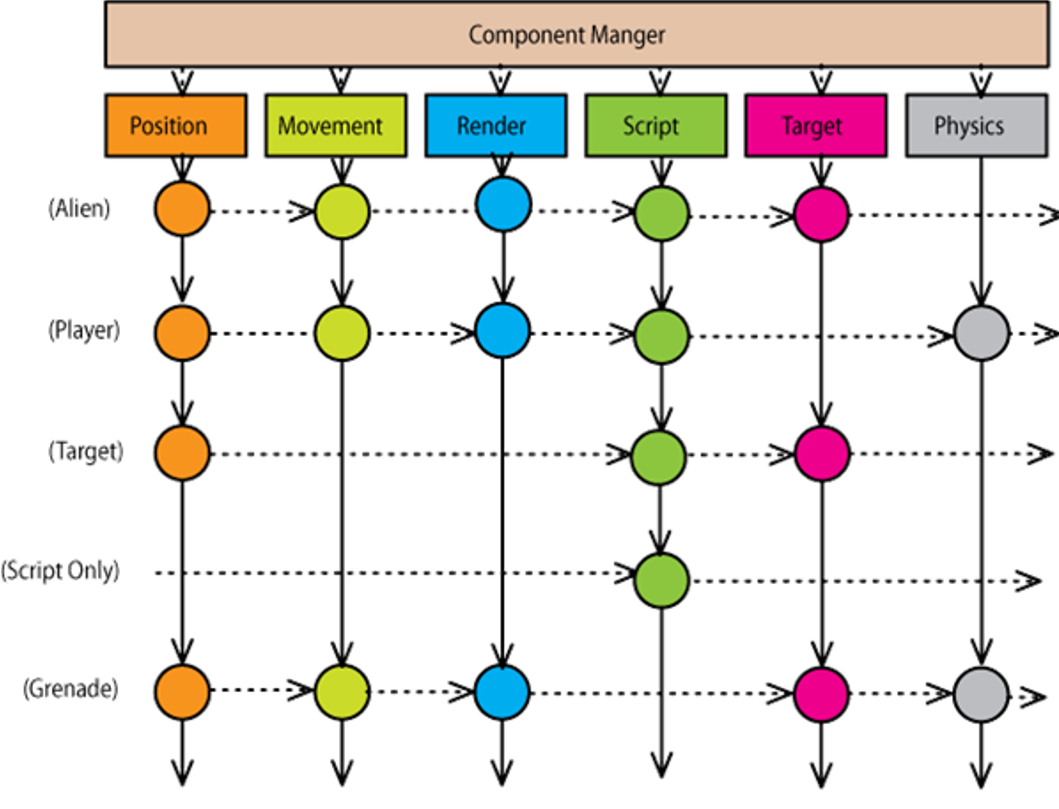
\includegraphics[width=0.5\textwidth]{img/ECSComponentManager.png}
	\caption{ECS Component manager}
	Source: \autocite{img:ECSComponentSystem}
	\label{fig:ECS Component manager}
\end{figure}

Another aspect that makes the \gls{ecs} very fast, is that a system can handle all
components (of the same type) together at once. This is possible because all entities
are independent of each other.

There are many ways of implementing the systems. Some say that each component type
has their own system. This interpretation of the systems does not take the interplay
of different component types, into account. A less restrictive approach is to let
different systems deal with all components they should be concerned with. For
instance a Physics Systems should be aware of Collision Components and Rigidbody
Components, as both probably contain necessary information regarding physics
simulation. It's best to see systems as ``closed environments''. That is, they do not
take ownership of entities nor components. They do access them through independent
manager objects, which in turn will take care of the entities and components
life-cycle \autocite{man:ECSExplanation}.

Sometimes systems, entities and even components need to cummincate with each other.
This might be very hard because systems, entities and components are more or less
independent. One option is to use an event systems. A system, entity and component
can raise an event and other systems, entities and components can react to that
event. This is what makes the \gls{ecs} a complicated system (disadvantage)
\autocite{man:ECSExplanation}.

There are many C/C++ libraries available, completely dedicated to \gls{ecs}. The most
popular libraries are shown in \cref{tab:popularECSLibraries}. The popularity is
based on the amount of stars on GitHub.

\begin{table}
	\centering
	\begin{tabular}{ll@{\qquad}lr}
		\toprule
		\textbf{Name} & \textbf{Short Description} & \textbf{Stars} & \textbf{License}\\
		\midrule
		EnTT & Fast and reliable entity-component system & 10k & MIT\\
		Flecs & A Multithreaded Entity Component System & 6.3k & MIT\\
		EntityX & Fast, type-safe C++ entity component system & 2.2k & MIT\\
		\bottomrule
	\end{tabular}
	\caption{Popular \glsfmtname{ecs} libraries}
	Source: \autocite{github:awesome-ecs}
	\label{tab:popularECSLibraries}
\end{table}

TODO: Add library benchmark to find the best library.

It is, of course, not necessary to use a library to implement an \gls{ecs}
architecture. However, it seems very hard to achieve the same performance as a
library \autocite{github:ecsfaq}.

% \subsection{Conclusion}

\section{Gameobjects/components}
\label{sec:gameobjects-components}

\subsection{Introduction}

One of the requirements of our customer, is that the game engine's structure is
similar to Unity. The customer has created a class diagram of the game engine's API,
which is (of course) very similar to Unity. One of the most important parts of the
class diagram is a so-called gameObject (with several components). It's needed to
understand the exact meaning/function of these gameObjects, that's why this research
question arose.

\subsection{Findings}

A gameObject is the most important concept in Unity. Every object in a game is a
GameObject, from characters and collectible items to the lights, cameras and special
effects. However, a gameObject itself can't do anything on its own. A gameObject
needs to be given properties before it can become a character, an envirnment, or a
special effect. \autocite{man:unityGameobjects}

A gameObject can be seen as a container for components. Components are the properties
of the gameObject. A few examples of components are sprites, animators, audioSources,
and so on. Multiple (different) components can be assigned to a single gameObject
(e.g.~a sprite and an audioSource).

Since we now know that a gameObject needs components to do something, it's obvious
that there should be a way to add components to a gameObject. Some components
(e.g.~the behaviorScript component) should also be able to reference to its
gameObject.

Each gameObject always has one transform class. The transform class describes the
position, rotation, and scale within the scene. Some component use this information
to e.g.~scale a sprite. Other components eddit this information to e.g.~model
gravity. \autocite{man:unityTransformClass}

A gameObject can have one (or multiple) children gameObject(s). All children
gameObjects, of course, also have one transform class. However, the position,
rotation, and scale of this class, is always the same as the child's parent. A child
can not have more than one parent. \autocite{man:unityTransformClass}

\subsection{Conclusion}

\section{Third-party tools}

\subsection{Introduction}

Developing a game engine from scratch requires a significant amount of time, as many
different features are necessary. Fortunately, some of these features have already
been developed and can be reused in the form of frameworks and third-party
tools/libraries. The decision to use third-party libraries, and the selection of
which ones to use, directly influences the development process of the game engine. In
this section, several third-party frameworks and tools available for use are
described.

\subsection{Findings}

\subsubsection{Media frameworks}

A game engine must have the ability to handle user input, render graphics, and
process audio. Several large frameworks are available that provide these features and
are already widely used by other game engines. The two most popular and
best-supported options are \gls{sdl2} and \gls{sfml}.

\paragraph{SDL2}

% TODO: ref?sdl2
According to its official website, \gls{sdl2} is \emph{``a cross-platform development
library designed to provide low-level access to audio, keyboard, mouse, joystick, and
graphics hardware via \gls{opengl} and \gls{d3d}. It is used by video playback
software, emulators, and popular games, including Valve's award-winning catalog and
many Humble Bundle games.''} \gls{sdl2} is written in the C programming language, and
therefore, structs and functions are used instead of objects and methods.

\begin{comparison}
	\pro{Controller support is provided.}
	\pro{2D and 3D rendering are supported.}
	\pro{Broad multiplatform support is offered, including older consoles such as the
	Wii.}
	\pro{Low-level control is available.}
	\pro{A large community ensures wide usage.}
	\pro{Extended libraries can be used to add functionalities, such as SDL\_Mixer for
	sound.}
	\con{A limited built-in 2D renderer is provided.}
	\con{Extended libraries require setup.}
\end{comparison}

\paragraph{SFML}

\gls{sfml} is a simple framework consisting of five modules: audio, graphics,
network, system, and window. This framework, written in C++, was designed to simplify
game development.

\begin{comparison}
	\pro{Object-oriented design is provided since it is written in C++.}
	\pro{A built-in 2D renderer is available for ease of use.}
	\pro{A built-in audio system is included.}
	\pro{Cross-platform support is available for Linux, Windows, and macOS.}
	\pro{Networking capabilities are provided for multiplayer or networked
	applications.}
	\con{The 2D rendering engine may experience performance issues in large-scale
	games.}
	\con{The community is smaller compared to \gls{sdl2}.}
	\con{No native 3D support is provided.}
	\con{Not all image formats are supported.}
\end{comparison}

\subsubsection{Audio}

for audio some options could be: FMOD, Wwise, or iirKlang

\subsection{Conclusion}

\section{Resource manager}

\subsection{Introduction}

\subsection{Findings}

\subsection{Unity formats}

% TODO: +ref (urldate 2024-09-11)
Unity has many different asset file types that can be imported to use for a game
\href{https://docs.unity3d.com/Manual/BuiltInImporters.html}{unity imports}. The most
important formats are the audio, text and sprite formats.

\subsubsection{Audio}

% NOTE: multicols to save space (is this list necessary?)
The unity engine supports a lot of different audio formats:\noparbreak
\begin{multicols}{5}
\begin{itemize}
	\item ogg.
	\item aif.
	\item aiff.
	\item flac.
	\item wav.
	\item mp3.
	\item mod.
	\item it.
	\item s3m.
	\item xm.
\end{itemize}
\end{multicols}

\subsubsection{Sprite formats}

% NOTE: multicols to save space (is this list necessary?)
Unity supports many different image formats:\noparbreak
\begin{multicols}{5}
\begin{itemize}
	\item jpg.
	\item jpeg.
	\item tif/tiff.
	\item tga.
	\item gif.
	\item png.
	\item psd.
	\item bmp.
	\item iff.
	\item pict.
	\item pic.
	\item pct.
	\item exr.
	\item hdr.
\end{itemize}
\end{multicols}

\subsection{Audio format}

% TODO: +ref (both urldate 2024-09-12)
The choice of audio format for the cr\^epe game engine depends on several factors,
including sound quality, memory usage, and licensing. According to various sources
\href{https://dev.to/tenry/comparison-of-audio-formats-for-games-jak}{comparison audio formats},
\href{https://www.universityofgames.net/articles/audio-file-formats-used-in-game-development/}{Audio files in games},
the most commonly used audio formats in game development are WAV, MP3, and Ogg.

\subsubsection{Licensing}

Historically, MP3 had patents on the audio format, but these restrictions have
expired. Ogg and FLAC, both developed by Xiph.Org, are open-source formats.
Additionally, the WAV format, though widely used, does not require a specific license
for distribution.

\subsubsection{Conclusion}

For the cr\^epe game engine, Ogg and FLAC are the preferred audio formats due to
their open-source licenses and high compatibility. FLAC is ideal for high-quality
audio with minimal compression, while Ogg is better suited for lower-quality audio
that requires reduced memory usage. Both formats come from the same non-profit
organization, Xiph.Org, ensuring that they align with open-source values and
licensing flexibility.

\subsection{Conclusion}

% \section{Rendering}
% 
% \subsection{Introduction}
% 
% \subsection{Findings}
% 
% \subsection{Conclusion}

% \section{Event manager/game loop}
% 
% \subsection{Introduction}
% 
% \subsection{Findings}
% 
% \subsection{Conclusion}

% % TODO: this entire section
% \section{Profiling and debugging}
% 
% % Which profiling and debugging features are wanted?
% % How to provide those profiling and debugging features?
% % Can most of the profiling/debugging be handled by external tools?
% 
% % Ideas:
% % - flame graph
% % - watchtable (combine w/ fps/speed control overlay?)
% % - debug printing utility functions
% 
% \subsection{Introduction}
% 
% \subsection{Findings}
% 
% \subsubsection{Callgrind}
% 
% \begin{comparison}
% 	\pro{Source code does not need to be modified for profiling}
% 	\con{Execution speed is severely impacted}
% \end{comparison}
% 
% \subsection{Conclusion}

\section{Physics}

%links
%ragdoll info: https://learn.unity.com/tutorial/creating-ragdolls-2019#649c42abedbc2a04c2145ce7
%softbody info: https://www.greenfoot.org/scenarios/29502

%2d box concepts: https://box2d.org/
%liquidfun (fork of box2d): https://google.github.io/liquidfun/
%Chipmunk2D: https://chipmunk-physics.net/
% particel systemhttps://learn.unity.com/tutorial/introduction-to-particle-systems#
%rigid body:https://docs.unity3d.com/ScriptReference/Rigidbody.html

\subsection{Introduction}

This part of the research explains Physics concepts and the use of physics in a game
engine. Furthermore, it examines the ease of using a physics engine compared to
implementing physics from scratch. Ultimately, a recommendation will be provided on
whether using a physics engine is more feasible than a custom implementation.

\subsection{Physics concepts}

Some information about certain Physics topics. second partdescibes what physics we
will be able to use and what it is.

%Physics core concepts: https://bluebirdinternational.com/game-physics/#:~:text=Game%20physics%20is%20implemented%20using,solid%20and%20deformable%20objects%2C%20respectively

%ragdoll https://bluebirdinternational.com/ragdoll-physics/

\begin{description}
	\item[Kinematics] Kinematics in game physics involves calculating the position,
		velocity, and acceleration of objects to simulate realistic motion. It affects
		everything from character movement to projectiles and vehicles. Collision
		detection is key, as it determines when objects collide and how they respond,
		including any damage or effects. Kinematics also helps create lifelike
		animations, like jumping or running, enhancing the game's realism and immersion.
		\begin{itemize}
			\item mass
			\item speed
			\item direction
			\item collision detection
		\end{itemize}
	\item[Dynamics] Dynamics simulate object interactions and forces, such as gravity
		and friction, to enhance realism. It includes rigid body, soft body, and fluid
		dynamics. For example, it affects car movements in racing games and projectiles
		in shooters. Balancing dynamics is crucial to maintain performance. Ragdoll
		physics, a related concept, models a character's body as interconnected rigid
		bodies for realistic movement.
		\begin{itemize}
			\item rigid body dynamics
			\item soft body dynamics
			\item fluid dynamics
			\item ragdoll physics
		\end{itemize}
	\item[Collision] Collision detection is the process of determining when two or more
		objects in the game world come into contact with each other. There are several
		techniques used for collision detection.
		\begin{itemize}
			\item bounding boxes
			\item bounding spheres
			\item mesh-based collision
		\end{itemize}
		These techniques involve creating simple shapes around the objects and checking
		if they intersect with each other.
	\item[Rigidbody] Rigidbodys deels with the behavior of of non deformable solid
		objects. it has some physical properties.
		\begin{itemize}
			\item mass
			\item velocity
			\item angular velocity
			\item orientation
		\end{itemize}
		To calculate all forces applied to the rigid body the most used algoritm is
		Newton-Euler equations. The alogritm is about mass an conservation of energy.
	\item[Softbody] Soft body dynamics simulates deformable objects like cloth, fluids,
		and flesh, adding complexity beyond rigid body dynamics. Key techniques
		include:\noparbreak
		\begin{itemize}
			\item Finite Element Method: Divides the object into small elements that
				interact based on physical laws.
			\item Mass-Spring Systems: Uses masses and springs to model deformation and
				stretching.
		\end{itemize}
		These methods enhance game realism by creating lifelike clothing, natural water
		effects, and realistic collision deformations. However, they are resource
		intensive an require precise calculations to avoid unrealistic results.
		\item[Particle Systems] Particle systems simulate numerous small objects to
			create larger effects like dust, smoke, fire, or explosions. These effects can
			add an extra layer of realism to a game.
		\item[Fluid Dynamics] Fluid dynamics shows how fluids move and behave. In game
			physics, it simulates liquids like water or lava, adding complexity and realism
			to games with fluid interactions.
		\item[Aerodynamics] Aerodynamics shows the movement of air and its interaction
			with solid objects. In video games, it simulates how objects like airplanes or
			birds move through the air, adding a realistic touch to games involving flight
			or gliding.
\end{description}

\subsection{Findings}

This part shows some phiscics engines an certain physics features that could be
needed within the project.

\subsubsection{Available physics engines}

Available physics engines for complex physics:\noparbreak
\begin{description}
	\item[Box2D] One of the most popular and widely used open-source 2D physics
		engines, Box2D is known for its simplicity, robustness, and efficiency.

		MIT licensed.
	\item[LiquidFun] A fork of Box2D, LiquidFun adds particle-based fluid simulation to
		Box2D's rigid body dynamics. It's ideal for games that require both solid and
		fluid dynamics.

		Apache 2.0 licensed.
	\item[Chipmunk2D] A lightweight and fast 2D physics engine that emphasizes ease of
		use and flexibility. Chipmunk2D is designed to be simple enough to understand and
		integrate but powerful enough for complex simulations.

		MIT licensed.
\end{description}

\subsubsection{Physics system (engine specific physics engine)}

A physics engine that is independent can be used across multiple game engines or
applications. But when the physics engine is built directly into the game engine and
can not be reused independently, it is often considered a physics system or physics
module within that specific engine. It is optimized and designed to work within the
constraints and features of that particular engine.

features a physics engine should provide is determined by the requirements. Because
the only requirement is that the user should easily add physics a list below is made
for simple physics that can be implemented without the use of an 3rd party physics
engine. Other features can be made by the user using scripts.

For simple features as listed below (besides collision and particels) a Physics
system is sufficient to provide these features to the game engine.

Simple Physics features a physics engine could provide:\noparbreak
\begin{itemize}
	\item Gravity
	\item Collision (detection + standard handeling)
	\item Rigidbody body\noparbreak
	\begin{itemize}
		\item mass
		\item gravity scale
		\item velocity
		\item body type\noparbreak
		\begin{itemize}
			\item Static
			\item Dynamic
			\item Kinematic (User script)
			\item Kinematic (standard)
		\end{itemize}
	\end{itemize}
	\item collsion detection mode
	\item movement\noparbreak
	\begin{itemize}
		\item player movement
		\item bounce
		\item rotation
		\item directional force
	\end{itemize}
	\item particels
\end{itemize}

\subsubsection{Physics with EC}

with EC the component (e.g.~Rigidbody) would have some functionality to change its
own physics. Besides storing data it would hold function as well for applying
gravity, forces, or handle other physics-related logic.

Preview of Rigidbody\noparbreak
\begin{itemize}
	\item Mass (data)
	\item gravityscale (data)
	\item velocity (data)
	\item applygravity (function)
	\item update position (function)
\end{itemize}

With this logic inside of each component the gameloop would look like this:

\begin{enumerate}[label={step \arabic*:},leftmargin=5em]
	\item Have a list of components.
	\item call for each component the rigidbody with the update function (changing its
		velocity)
	\item call for each component the update position function (change x and y of each
		entity)
	\item check for collsion handeling (would be the collsion component)
\end{enumerate}

Because it is not known with EC if the list contains all object with a rigidbody some
overhead is created if the entity does not have a component of the type rigidbody.

\subsubsection{Physics with ECS}

With ECS the component (e.g.~Rigidbody) would only be used to store data. all
functionality would be moved to the Physics system

Preview of Rigidbody
\begin{itemize}
	\item Mass (data)
	\item gravityscale (data)
	\item velocity (data)
\end{itemize}

Preview of physics system
\begin{itemize}
	\item applygravity (function)
	\item update position (function)
\end{itemize}

A seperate sytem would be made that would do all the calculations for the physics.

With this logic inside of each component the gameloop would look like
this:\noparbreak
\begin{enumerate}[label={Step(\arabic*):},leftmargin=5em]
	\item ECS provides a list of rigidbodies (with the enitties)
	\item physics system updates all components
\end{enumerate}

The benefit of ECS is that all physics and collsions are handled by one system. The
Physics functionalities would be gathered in one place instead of multiple
components. The Physics system could seperate the Physics function creating a correct
Physics flow with only one loop. For EC to do this each function would need to have
its own loop in the gameloop creating more overhead.

What EC can not provide compared to ECS is a physics world. A physics world would be
the physics that apply to all dynamic physics components. If you want to create
gravity you can add the force to the world. The physics system would read all the
Physics forces in the world and apply them to all dynamic entities. This would create
an easier to use interface for the user and improve the efficiency of the physics
because the total forces can be calcualted ones and then applied to all dynamic
entities.

\subsection{Conclusion}

More components need te be created for both EC and ECS with the diagram provided by
the customer. With ECS having the benefit of creating a world where all dynamic
object can have a force they interact with. A physics system has the benefit that all
physics functionalities are located within one system instead in each component. The
flow of Physics updates can be change within the physics system instead of in the
gameloop itself.

\section{Collisions}

\subsection{Introduction}

Collision is mostly made part of an Physics engine, however it is something seperate
but some collision handeling is done by the Physics engine that is the reason why
they are most of the time one system.

Collsions exists from two thing. Collsion detection and collsion handeling/ Some
handeling is done by the physics engine and by user scripts and will not be
explanined in this topic. Collsion detection is the scope of this research. There is
a need of understanding what different type of collision objects are and what
algoritm can be used to increase efficiency of the detection.

\subsection{Findings}

Collsion detection is made out of 2 fases.

%https://developer.mozilla.org/en-US/docs/Games/Techniques/2D_collision_detection

%https://medium.com/@bpmw/quadtrees-for-2d-games-with-moving-elements-63360b08329f

%https://medium.com/my-games-company/optimizing-r-tree-inserts-in-unity-a-bomberman-like-example-81d2576efd75

%https://matthias-research.github.io/pages/tenMinutePhysics/11-hashing.pdf

The first fase want to make a list out of objects that could be colliding. Some
algorithm can be used to make these list in an efficient way. quadtrees, R-Trees or
a spatial hashmap.

\begin{description}
	\item[Quadtrees] Quadtrees partition 2D space into quadrants (stored as nodes in a
		tree), dividing these quadrants into smaller quadrants when they contain more
		than a certain threshold of elements.
	\item[R-Trees] These are data structures commonly used for spatial access. They are
		more suited for dynamic data and allow efficient querying of rectangles or
		bounding boxes, making them useful for collision detection.
	\item[Spatial hashing] This technique divides space into uniform grids (similar to
		cells in a 2D array), and each object is assigned to one or more cells based on
		its position. Objects within the same or adjacent cells are checked for
		collisions, improving efficiency by limiting the number of checks to nearby
		objects.
\end{description}

R-Trees are easy to understand but how the R-tree is build (how objects are inserted)
is complex. The benefits of this tree for this project are not needed because
quadtree would be sufficient for this purpose. reading the data would be as fast as
the quadtree but implemeting the R-tree and knowing how to implement it takes to much
time and is out of scope.

\begin{table}
	\begin{tabularx}{\linewidth}{p{8em}XXX}
		\toprule
		Criteria & Quadtree & R-tree & Spatial hashing \\
		\midrule
		Best for & Static objects, sparse data & Complex shapes, dynamic objects & Fast-moving objects, uniform data \\
		\midrule
		Handles moving objects & Poorly (requires restructuring) & Well (efficient updates) & Very well (simple re-hash) \\
		\midrule
		Memory usage & Moderate & Moderate to high & Can be high \\
		\midrule
		Complexity & Moderate & High & Low \\
		\midrule
		Spatial queries & Efficient & Very efficient & Less efficient \\
		\midrule
		Grid size sensitivity & N/A & N/A & High (tuning needed) \\
		\midrule
		Handling variable density & Good & Good & Poor \\
		\bottomrule
	\end{tabularx}
	\caption{Comparison of quadtree, R-tree, and spatial hashing}
\end{table}

%https://developer.mozilla.org/en-US/docs/Games/Techniques/2D_collision_detection

The second face checks the list from the first face if there are actually colliding. the narrow face detections are descripted in the list below.

List of collision detection objects/algoritms (narrow)
\begin{description}
	\item[Axis-Aligned Bounding Box]One of the simpler forms of collision detection is
		between two rectangles that are axis aligned --- meaning no rotation. The
		algorithm works by ensuring there is no gap between any of the 4 sides of the
		rectangles.
	\item[Circle Collision] a simple shape for collision detection is between two
		circles. This algorithm works by taking the center points of the two circles and
		ensuring the distance between the center points are less than the two radii added
		together.
	\item[Separating Axis Theorem] This is a collision algorithm that can detect a
		collision between any two convex polygons. It's more complicated to implement
		than other methods but is more powerful.
\end{description}

\subsection{Conclusion}

% \section{Audio}
% 
% \subsection{Introduction}
% 
% \subsection{Findings}
% 
% \subsection{Conclusion}

% \section{AI}
% 
% \subsection{Introduction}
% 
% \subsection{Findings}
% 
% \subsection{Conclusion}

\end{document}

